\part{Capítulo 9}
Los esfuerzos que toma y transmite la fundación al suelo de apoyo están relacionados al tipo de estructura de que se trate y su uso:
\begin{itemize}
    \item Esfuerzos normales uniformes y constantes
    \item Esfuerzos normales uniformes y variables
    \item Esfuerzos preferencialmente oblicuos
    \item Esfuerzos preferencialmente horizontales
    \item Esfuerzos normales no uniformes
    \item Esfuerzos cíclicos
\end{itemize}

Una fundación puede fallar en varias formas y el grado de daño que sufre la supraestructura debido a tales fallas se clasifican como sigue:
\begin{itemize}
    \item Asentamientos
    \item Volcamiento
    \item Deslizamiento
\end{itemize}

\subsection{Características del Suelo de fundación}
Existe una variedad de suelos que pueden ir de roca al légamo (limo de fondos pantanoso):
\begin{itemize}
    \item Roca: ígnea y eruptiva, sedimentaria y metamórfica
    \item Grava y suelos de Grava
    \item Arenas y suelos de arena
    \item Suelos de grano fino con poca plasticidad
    \item Suelos de grano fino con media a alta plasticidad
    \item Material de suelo inadecuado: con poder de soporte inferior a 3\% CBR (California Bearing Ratio)
    \begin{itemize}
        \item Suelo heladizo
        \item Capa vegetal
        \item Material cuyo porcentae de expansión sea mayor que 3\%
        \item Suelos salinos naturalmente cementados
    \end{itemize}
    \item Agua subterránea
    \begin{itemize}
        \item Puede tener consecuencias tanto en la capacidad de soporte de los suelos, como en los mayores costos, asociados a un diseño del proyecto de fundación más conservador.
    \end{itemize}
\end{itemize}

\subsection{Tipos de fundación}
\begin{itemize}
    \item Fundaciones superficiales
    \begin{itemize}
        \item Zapatas Aisladas
        \item Zapatas atirantadas
        \item Zapata y Viga de fundación
        \item Zapata corrida
        \item Losa de fundación
        \item Losa Flotante
    \end{itemize}
    \item Fundaciones profundas
    \begin{itemize}
        \item Pilotes
        \item De Cajón
        \item Otras
    \end{itemize}
    \item Fundaciones de máquinas
\end{itemize}

\subsection{Fundaciones superficiales}
\begin{itemize}
    \item Considerar como mínimo 60 a 80 cm, empotrando al menos 20 a 30cm en estrato competente
    \item Debe asegurar un $FS \geq 3$ al hundimiento
    \item Debe ser suficiente como para que la cota de cimentación no se vea afectada por la T° o la humedad
    \item Debe considerar la profundidad de socavación
    \item Debe absorber o limitar de buena manera los asentamientos diferenciales y distorsiones angulares
\end{itemize}
\begin{figure}[h]
    \centering
    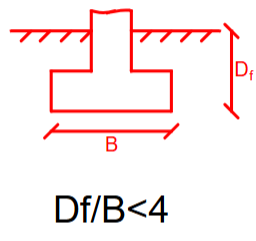
\includegraphics[width=0.3\textwidth]{FOTOS/sello_cimentacion.png}
    \caption{Sello de cimentación}
    \label{fig:9_1}    
\end{figure}

\newpage
\begin{itemize}
    \item Maquinaria sensible a deformaciones $\Delta /L < 1/750 a 1/3000$
    \item Estructuras de hormigón armado $\Delta /L < 1/500$
    \item Pórticos con diagonales $\Delta /L < 1/600$
    \item Dificultades en grúas $\Delta /L < 1/300$
    \item Inclinación visible en edificios $\Delta /L < 1/250$
    \item Daños estructurales $\Delta /L < 1/150$
\end{itemize}

\begin{figure}[h]
    \centering
    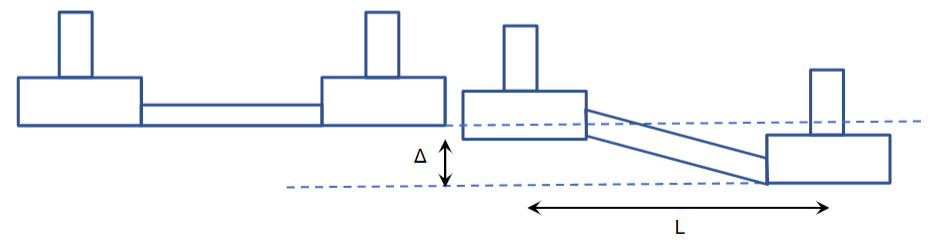
\includegraphics[width=0.5\textwidth]{FOTOS/sello_cimentacion2.png}
    \caption{Sello de cimentación}
    \label{fig:9_2}
\end{figure}

\subsection{Fundaciones profundas}
\begin{itemize}
    \item Miembros estructurales hechos de acero, hormigón o madera
    \item Sistema más costoso que fundación superficial
    \item A veces es necesario su uso para garantizar seguridad estructural:
    \begin{itemize}
        \item Transmición de cargas
        \item Esfuerzos horizontales
        \item Suelos difíciles
        \item Pilas de puentes
    \end{itemize}
\end{itemize}

\begin{figure}[h]
    \centering
    \includegraphics[width=0.3\textwidth]{FOTOS/pilotes.png}
    \caption{Pilotes}
    \label{fig:9_3}
\end{figure}

\begin{itemize}
    \item Según transmición de cargas al suelo
    \begin{itemize}
        \item Pilotes de punta
        \item Pilotes de fricción
        \item Pilotes de compactación
    \end{itemize}
    \item Según sistema constructivo
    \begin{itemize}
        \item Pilotes hincados
        \item Pilotes perforados
        \begin{itemize}
            \item Con camisa
            \item Sin camisa
        \end{itemize}
    \end{itemize}
\end{itemize}

\subsection{Fundaciones de máquinas}
\begin{itemize}
    \item Las máquinas son sensibles a los cambios de nivel o asentamientos
    \item Es conveniente usar aisladores en unión con las máquinas para evitar transmitancia de vibraciones
    \item Las fundaciones deben impedir que las vibraciones en ellas por las máquinas sean excesivas. El peso de las fundaciones puede varias de 2 a 10 veces el peso de una máquina
\end{itemize}

\subsection{Aisladas sísmicamente}
Los aisladores sísmicos friccionales consisten en un conjunto de láminas de goma natural y acero, colocadas alternadamente y adheridas entre sí, para formar un dispositivo con una gran flexibilidad horizontal y una gran rigidez vertical 

Esta tecnología puede resultar en un costo mayor al valor del edificio, que rodea entre el 3 y el 5\%. Es una buena medida especialmente para edificios en hormigón con proyección de uso de 50 años o más